% \documentclass[table]{beamer}
\documentclass[table,handout]{beamer}
\setbeameroption{show notes}
% \setbeameroption{hide notes}
% \setbeameroption{show only notes}
\usepackage{varwidth}

\newif\ifhide
\newif\ifpost
\newif\ifhideclicker

% \hidetrue
% \hideclickertrue
% \posttrue

\newcommand{\whiteout}[1]{\textcolor{white}{#1}}
% \newcommand{\whiteoutbox}[1]{\fcolorbox{white}{white}{\parbox{\dimexpr \linewidth-2\fboxsep-2\fboxrule}{\whiteout{#1}}}}
% \newcommand{\notebox}[1]{\fcolorbox{blue}{white}{\parbox{\dimexpr \linewidth-2\fboxsep-2\fboxrule}{#1}}}
\newcommand{\whiteoutbox}[1]{\fcolorbox{white}{white}{\parbox{\linewidth}{\whiteout{#1}}}}
\newcommand{\notebox}[1]{\fcolorbox{blue}{white}{\parbox{\linewidth}{#1}}}
\newcommand{\blankbox}[1]{\phantom{\varwidth{\linewidth}\whiteoutbox{#1}\endvarwidth}}
\newcommand{\blank}[1]{\phantom{\varwidth{\linewidth}#1\endvarwidth}}

\ifhide%
    \newcommand{\hmask}[1]{\blank{#1}}%
\else%
    \newcommand{\hmask}[1]{#1}%
\fi

\ifhide%
    \newcommand{\wout}[1]{\whiteout{#1}}%
\else%
    \newcommand{\wout}[1]{#1}%
\fi

\ifhide%
    \newcommand{\hignore}[1]{}%
\else%
    \newcommand{\hignore}[1]{#1}%
\fi

\ifpost%
    \newcommand{\nopost}[1]{}%
\else%
    \newcommand{\nopost}[1]{#1}%
\fi

\ifhideclicker%
    \newcommand{\clickerslide}[1]{\stepcounter{clickerQuestionCounter}%
        \begin{frame}[t]
            \textcolor{blue}{Q \arabic{clickerQuestionCounter}:}
        \end{frame}}
\else%
    \newcommand{\clickerslide}[1]{#1}%
\fi

\ifhide%
    \newcommand{\hidebox}[1]{\blank{#1}}%
\else%
    \newcommand{\hidebox}[1]{\notebox{#1}}%
\fi

\ifhide%
    \newcommand{\wbox}[1]{\whiteoutbox{#1}}%
\else%
    \newcommand{\wbox}[1]{\notebox{#1}}%
\fi

\ifhide%
    \newcommand{\nbox}[1]{\blankbox{#1}}%
\else%
    \newcommand{\nbox}[1]{\notebox{#1}}%
\fi

\ifhideclicker%
    \newcommand{\clickeranswer}[1]{#1}%
\else%
    \ifhide%
        \newcommand{\clickeranswer}[1]{#1}%
    \else%
        \newcommand{\clickeranswer}[1]{\textbf{\textcolor{blue}{#1}}}%
    \fi
\fi

\usepackage{beamerthemesplit}
% \usetheme{boxes}
\usetheme{Malmoe}
\usecolortheme{seahorse}
% \usecolortheme{seagull}
\usepackage{ifthen}
\usepackage{xspace}
\usepackage{multirow}
\usepackage{multicol}
\usepackage{booktabs}
\usepackage{xcolor}
\usepackage{wasysym}
\usepackage{comment}
\usepackage{hyperref}
\hypersetup{pdfborder={0 0 0}, colorlinks=true, urlcolor=blue, linkcolor=blue, citecolor=blue}
\usepackage{changepage}
\usepackage[compatibility=false]{caption}
\captionsetup[figure]{font=scriptsize, labelformat=empty, textformat=simple, justification=centering, skip=2pt}
\usepackage{tikz}
\usetikzlibrary{trees,calc,backgrounds}

\usepackage[bibstyle=joaks-slides,maxcitenames=3,mincitenames=1,backend=biber]{biblatex}

\newrobustcmd*{\shortfullcite}{\AtNextCite{\renewbibmacro{title}{}\renewbibmacro{in:}{}\renewbibmacro{number}{}}\fullcite}

\newrobustcmd*{\footlessfullcite}{\AtNextCite{\renewbibmacro{title}{}\renewbibmacro{in:}{}}\footfullcite}

% Make all footnotes smaller
% \renewcommand{\footnotesize}{\scriptsize}

\definecolor{myGray}{gray}{0.9}
\colorlet{rowred}{red!30!white}

\setbeamertemplate{blocks}[rounded][shadow=true]

\setbeamercolor{defaultcolor}{bg=structure!30!normal text.bg,fg=black}
\setbeamercolor{block body}{bg=structure!30!normal text.bg,fg=black}
\setbeamercolor{block title}{bg=structure!50!normal text.bg,fg=black}

\newenvironment<>{varblock}[2][\textwidth]{%
  \setlength{\textwidth}{#1}
  \begin{actionenv}#3%
    \def\insertblocktitle{#2}%
    \par%
    \usebeamertemplate{block begin}}
  {\par%
    \usebeamertemplate{block end}%
  \end{actionenv}}

\newenvironment{displaybox}[1][\textwidth]
{
    \centerline\bgroup\hfill
    \begin{beamerboxesrounded}[lower=defaultcolor,shadow=true,width=#1]{}
}
{
    \end{beamerboxesrounded}\hfill\egroup
}

\newenvironment{onlinebox}[1][4cm]
{
    \newbox\mybox
    \newdimen\myboxht
    \setbox\mybox\hbox\bgroup%
        \begin{beamerboxesrounded}[lower=defaultcolor,shadow=true,width=#1]{}
    \centering
}
{
    \end{beamerboxesrounded}\egroup
    \myboxht\ht\mybox
    \raisebox{-0.25\myboxht}{\usebox\mybox}\hspace{2pt}
}

\newenvironment{mydescription}{
    \begin{description}
        \setlength{\leftskip}{-1.5cm}}
    {\end{description}}

\newenvironment{myitemize}{
    \begin{itemize}
        \setlength{\leftskip}{-.3cm}}
    {\end{itemize}}

% footnote without a marker
\newcommand\barefootnote[1]{%
  \begingroup
  \renewcommand\thefootnote{}\footnote{#1}%
  \addtocounter{footnote}{-1}%
  \endgroup
}

% define formatting for footer
\newcommand{\myfootline}{%
    {\it
    \insertshorttitle
    \hspace*{\fill} 
    \insertshortauthor, \insertshortinstitute
    % \ifx\insertsubtitle\@empty\else, \insertshortsubtitle\fi
    \hspace*{\fill}
    \insertframenumber/\inserttotalframenumber}}

% set up footer
\setbeamertemplate{footline}{%
    \usebeamerfont{structure}
    \begin{beamercolorbox}[wd=\paperwidth,ht=2.25ex,dp=1ex]{frametitle}%
        % \Tiny\hspace*{4mm}\myfootline\hspace{4mm}
        \tiny\hspace*{4mm}\myfootline\hspace{4mm}
    \end{beamercolorbox}}

% remove navigation bar
\beamertemplatenavigationsymbolsempty

\makeatletter
    \newenvironment{noheadline}{
        \setbeamertemplate{headline}[default]
        \def\beamer@entrycode{\vspace*{-\headheight}}
    }{}
\makeatother

\newcounter{clickerQuestionCounter}
\ifhideclicker%
\newenvironment{clickerquestion}
{ \stepcounter{clickerQuestionCounter}
  \begin{enumerate}[Q \arabic{clickerQuestionCounter}:]\color{white} }
{ \end{enumerate} }
\else%
\newenvironment{clickerquestion}
{ \stepcounter{clickerQuestionCounter}
  \begin{enumerate}[Q \arabic{clickerQuestionCounter}:] }
{ \end{enumerate} }
\fi

\ifhideclicker%
\newenvironment{clickeroptions}
{ \begin{enumerate}[\begingroup\color{white} 1)\endgroup]\color{white} }
{ \end{enumerate} }
\else%
\newenvironment{clickeroptions}
{ \begin{enumerate}[\begingroup\color{red} 1)\endgroup] }
{ \end{enumerate} }
\fi


\tikzstyle{centered} = [align=center, text centered, font=\sffamily\bfseries]
\tikzstyle{skip} = [centered, inner sep=0pt, fill]
\tikzstyle{empty} = [centered, inner sep=0pt]
\tikzstyle{inode} = [centered, circle, minimum width=4pt, fill=black, inner sep=0pt]
\tikzstyle{tnode} = [centered, circle, inner sep=1pt]
\tikzset{
  % edge styles
  level distance=10mm,
  mate/.style={edge from parent/.style={draw,distance=3pt}},
  mleft/.style={grow=left, level distance=10mm, edge from parent path={(\tikzparentnode.west)--(\tikzchildnode.east)}},
  mright/.style={grow=right, level distance=10mm, edge from parent path={(\tikzparentnode.east)--(\tikzchildnode.west)}},
  % node styles
  male/.style={rectangle,minimum size=4mm,fill=gray!80},
  female/.style={circle,minimum size=4mm,fill=gray!80},
  amale/.style={male,fill=red},
  afemale/.style={female,fill=red},
}

\newcommand{\highlight}[1]{\textcolor{violet}{\textit{\textbf{#1}}}}
\newcommand{\super}[1]{\ensuremath{^{\textrm{\sffamily #1}}}}
\newcommand{\sub}[1]{\ensuremath{_{\textrm{\sffamily #1}}}}
\newcommand{\dC}{\ensuremath{^\circ{\textrm{C}}}}
\newcommand{\tb}{\hspace{2em}}
\providecommand{\e}[1]{\ensuremath{\times 10^{#1}}}
\newcommand{\myHangIndent}{\hangindent=5mm}

\newcommand{\spp}[1]{\textit{#1}}

\newcommand\mybullet{\leavevmode%
\usebeamertemplate{itemize item}\hspace{.5em}}

\makeatletter
\newcommand*{\rom}[1]{\expandafter\@slowromancap\romannumeral #1@}
\makeatother

\newcommand{\blankslide}{{\setbeamercolor{background canvas}{bg=black}
\setbeamercolor{whitetext}{fg=white}
\begin{frame}<handout:0>[plain]
\end{frame}}}

\newcommand{\whiteslide}{
\begin{frame}<handout:0>[plain]
\end{frame}}

\newcommand{\f}[1]{\ensuremath{F_{#1}}}
\newcommand{\x}[1]{X\ensuremath{^{#1}}}
\newcommand{\y}[1]{Y\ensuremath{^{#1}}}

% Population growth macros
\newcommand{\popsize}[1]{\ensuremath{N_{#1}}}
\newcommand{\popgrowthratediscrete}[1]{\ensuremath{\lambda_{#1}}}
\newcommand{\popgrowthrate}[1]{\ensuremath{r_{#1}}}
\newcommand{\ptime}{\ensuremath{t}\xspace}

\tikzset{hide on/.code={\only<#1>{\color{white}}}}
\tikzset{
    invisible/.style={opacity=0},
    visible on/.style={alt={#1{}{invisible}}},
    alt/.code args={<#1>#2#3}{%
        \alt<#1>{\pgfkeysalso{#2}}{\pgfkeysalso{#3}}
        % \pgfkeysalso doesn't change the path
    },
}

% \bibliography{../bib/references}
\bibliography{references}
\author[J.\ Oaks]{
    %Jamie R.\ Oaks\inst{1}
    Jamie R.\ Oaks
}
\institute[BIOL 180]{
    \inst{}%
        BIOL 180: Introductory Biology
}



\title[Patterns of Selection]{Patterns of Natural Selection}
% \date{\today}
\date{April 22, 2015}

\begin{document}

\begin{noheadline}
\maketitle
\end{noheadline}

\nopost{
\begin{noheadline}
\begin{frame}[c]
    \vspace{-6mm}
    \begin{center} 
        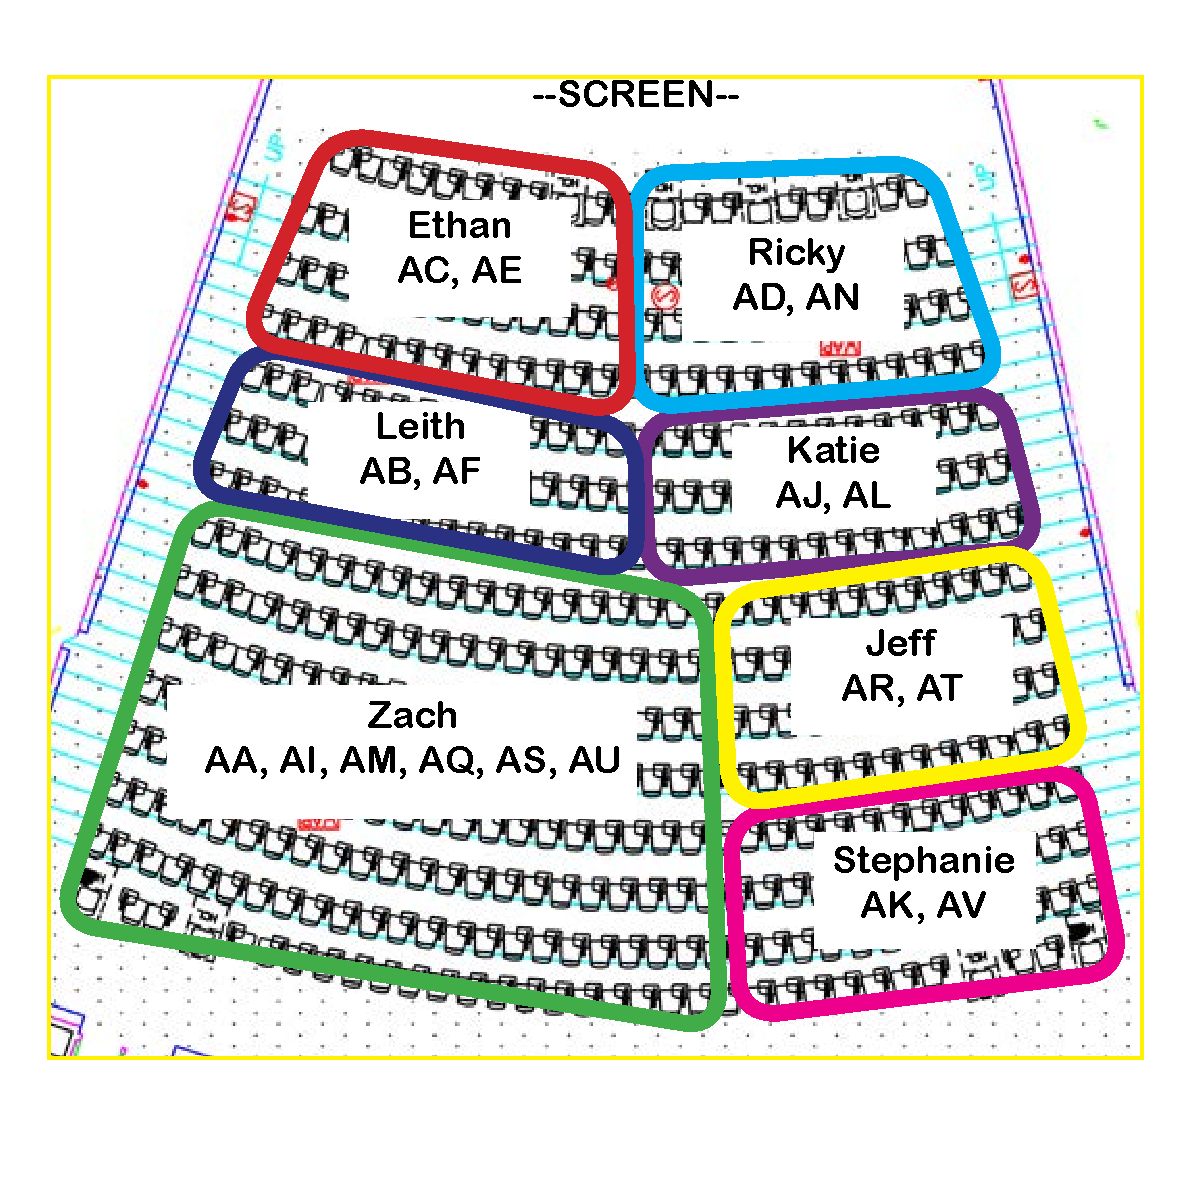
\includegraphics[height=1.2\textheight]{../images/seating-chart.pdf}
    \end{center}
\end{frame}
\end{noheadline}
}

\begin{noheadline}
\begin{frame}
\frametitle{Today's issues:}
\tableofcontents
\end{frame}
\end{noheadline}

\section{Applying the Hardy-Weinberg Principle}

\begin{frame}
\begin{adjustwidth}{-1.5em}{-1.5em}
Conclusions, under Hardy-Weinberg conditions: 

\begin{itemize}[<+->]
    \item If the allele frequencies in a population are given by $p$ and $q$,
        then the genotype frequencies are given by $p^2$, $2pq$, and $q^2$.

        \vspace{1cm}
    \item If the allele frequencies in a population are given by $p$, $q$, and
        $r$, then the genotype frequencies are given by $p^2$, $2pq$, $2pr$,
        $2qr$, $q^2$, and $r^2$. (And so on, for as many alleles as are
        present.)

        \vspace{1cm}
    \item When all individuals in the population breed and produce the same
        number of offspring, the allele frequencies in the population will not
        change, generation after generation. (They remain at p , q, and r
        forever.)
\end{itemize}

\end{adjustwidth}
% ``HW proportions'' ``HW equilibrium''
\end{frame}

\begin{frame}
\begin{adjustwidth}{-1.5em}{-1.5em}
    What are ``Hardy-Weinberg conditions'' with respect to the gene in question?
    
    \vspace{0.5cm}
    There is:
    \begin{itemize}
        \item \ \uncover<2->{No selection}
        \item \ \uncover<2->{No mutation}
        \item \ \uncover<2->{No gene flow}
        \item \ \uncover<2->{No genetic drift}
        \item \ \uncover<2->{Random mating}
    \end{itemize}

    \vspace{0.5cm}
    \uncover<2->{
    The Hardy-Weinberg principle furnishes a null model in population genetics.
    }

    \note[item]{pop gen = study of how allele frequencies change in
        populations}
    \note[item]{null = what to expect if no evolution is occurring}
    \note[item]{Do each assumption in terms of blonde hair---if all conditions
        met then genotype frequencies should be in HW proportions.}
\end{adjustwidth}
\end{frame}

\begin{frame}
    \small

    \begin{adjustwidth}{-1.5em}{-1.5em}
    \vspace{-0.2cm}
    \begin{columns}
        \column{0.5\textwidth}
    Problem 1: Survey 100 humans; determine genotypes at the $MN$ blood type
    locus.

        \column{0.5\textwidth}
    \begin{table}%[htbp]
        \small
        \centering
        \begin{tabular}{ p{1cm} p{1cm} p{1cm} }
            \toprule
            $MM$ & {$MN$} & {$NN$} \\
            \hline
            18 & 50 & 32 \\
            \bottomrule
        \end{tabular}
    \end{table}
    \end{columns}

    \vspace{2mm}
    \begin{enumerate}
            \small
        \item What is the observed frequency of the genotypes? 
            \nbox{\tiny $MM$: $18/100 = 0.18$; $MN$: $50/100 = 0.5$; $NN$: $32/100
                = 0.32$}

        \item What is the observed frequency of the $M$ and $N$ alleles?
        \begin{tabular}{ p{4cm} p{1cm} }
            $fr(M) = $ & $fr(N) = $ \\
        \end{tabular}
        \nbox{\tiny $fr(M) = ((18 \times 2) + 50)/200 = 86/200 = 0.43$
                    \hspace{1em}OR\hspace{1em}
                    $fr(M) = 0.18 + (0.5/2) = 0.43$ \\
            $fr(N) = ((32 \times 2) + 50)/200 = 114/200 = 0.57$
            \hspace{1em}OR\hspace{1em}
            $fr(M) = 0.32 + (0.5/2) = 0.57$}
        
        \item Given the observed allele frequencies, what are the expected
            genotype frequencies under the null hypothesis of no evolution and
            random mating with respect to the blood type gene?
            \nbox{\tiny   $fr(MM) = 0.43^2 = 0.185$ \\
                        $fr(MN) = 2(0.43)(0.57) = 0.49$ \\
                        $fr(NN) = 0.57^2$}

        \item Compare the observed and expected values: Do the data support the
            null hypothesis?
            \nbox{\tiny What kind of test should we use? Goodness-of-fit test}
    \end{enumerate}
    \end{adjustwidth}
\end{frame}

\begin{frame}[t]
    Problem 2: Survey a tapeworm population and determine genotype frequencies
    at an autosomal locus.
 
    \begin{table}%[htbp]
        % \addtolength{\tabcolsep}{-0.09cm}
        \centering
        \begin{tabular}{ p{1cm} p{1cm} p{1cm} }
            \toprule
            {$AA$} & {$Aa$} & {$aa$} \\
            \hline
            0.30 & 0.33 & 0.37 \\
            \bottomrule
        \end{tabular}
    \end{table}

    These are the \highlight{observed} frequencies of the genotypes.
\end{frame}

\clickerslide{
\begin{frame}[t]
    Problem 2: Survey a tapeworm population and determine genotype frequencies
    at an autosomal locus.
 
    \begin{table}%[htbp]
        % \addtolength{\tabcolsep}{-0.09cm}
        \centering
        \begin{tabular}{ p{1cm} p{1cm} p{1cm} }
            \toprule
            {$AA$} & {$Aa$} & {$aa$} \\
            \hline
            0.30 & 0.33 & 0.37 \\
            \bottomrule
        \end{tabular}
    \end{table}

    \begin{clickerquestion}
        \item What is the \highlight{observed} frequency of the $A$ and $a$ allele?
    \end{clickerquestion}
    \begin{table}%[htbp]
        % \addtolength{\tabcolsep}{-0.09cm}
        \centering
        \begin{tabular}{ l l l }
            \toprule
             & {$fr(A)$} & {$fr(a)$} \\
            \hline
            \textcolor{red}{1)} & \clickeranswer{0.465} & \clickeranswer{0.535} \\ 
            \textcolor{red}{2)} & 0.548 & 0.453 \\ 
            \textcolor{red}{3)} & 0.630 & 0.370 \\ 
            \textcolor{red}{4)} & 0.485 & 0.515 \\ 
            \textcolor{red}{5)} & 0.392 & 0.608 \\ 
            \bottomrule
        \end{tabular}
    \end{table}
\end{frame}
}

\clickerslide{
\begin{frame}[t]
    Problem 2: Survey a tapeworm population and determine genotype frequencies
    at an autosomal locus.
 
    \begin{table}%[htbp]
        % \addtolength{\tabcolsep}{-0.09cm}
        \centering
        \begin{tabular}{ p{1cm} p{1cm} p{1cm} }
            \toprule
            {$AA$} & {$Aa$} & {$aa$} \\
            \hline
            0.30 & 0.33 & 0.37 \\
            \bottomrule
        \end{tabular}
    \end{table}

    \begin{clickerquestion}
        \item What is the \highlight{expected} genotype frequencies under the
            null hypothesis of no evolution and random mating?
    \end{clickerquestion}
    \begin{table}%[htbp]
        % \addtolength{\tabcolsep}{-0.09cm}
        \centering
        \begin{tabular}{ l l l l}
            \toprule
             & {$fr(AA)$} & {$fr(Aa)$} & {$fr(aa)$} \\
            \hline
            \textcolor{red}{1)} & 0.286 & 0.497 & 0.216 \\ 
            \textcolor{red}{2)} & 0.333 & 0.333 & 0.333 \\ 
            \textcolor{red}{3)} & \clickeranswer{ 0.216} & \clickeranswer{0.497} & \clickeranswer{0.286 } \\ 
            \textcolor{red}{4)} & 0.300 & 0.330 & 0.370 \\ 
            \bottomrule
        \end{tabular}
    \end{table}
\end{frame}
}

\clickerslide{
\begin{frame}
    \begin{clickerquestion}
        \item Compare the observed and expected values. Do the data support the
            null hypothesis?
        \begin{clickeroptions}
            \item Yes---they are virtually identical
            \item No---too many heterozygotes observed
            \item No---too few homozygotes observed
            \item \clickeranswer{No---too few heterozygotes observed}
        \end{clickeroptions}
    \end{clickerquestion}
\end{frame}
}

\begin{frame}
    NOTE: you're making a MAJOR shift in your thinking \ldots

    \vspace{0.5cm}
    \begin{enumerate}
        \item Evolution = change in \highlight{allele frequencies} in a
            population over time.
        \item When you work on population genetics, you need to predict the
            frequencies of genotypes from many thousands of matings in a
            population---NOT the frequencies of genotypes from a particular
            mating. 
    \end{enumerate}

    \vspace{0.5cm}
    \ldots change to ``\highlight{population thinking}''
\end{frame}

\begin{frame}
    Where have we been, and where are we going? 

    \vspace{0.5cm}
    First 3 weeks:
    \begin{enumerate}
        \item Introduction to evolution by natural selection   
        \item Inheritance of variation (independent assortment, chromosome
            theory, recombination)
    \end{enumerate}

    \vspace{0.5cm}
    For Exam 2: 
    \begin{enumerate}
        \item Focus on evolution as changes in \highlight{allele frequencies}
        \item Explore natural selection and other processes that can change
            allele frequencies and cause evolution
    \end{enumerate}
\end{frame}

\section{Selection on quantitative traits}

\begin{noheadline}
\begin{frame}
\frametitle{Today's issues:}
\tableofcontents[currentsection]
\end{frame}
\end{noheadline}

\begin{frame}[t]
\begin{adjustwidth}{-1.5em}{-1.5em}

    \centering{
    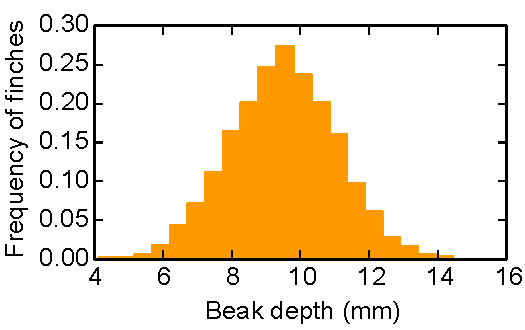
\includegraphics[width=0.6\textwidth]{../images/my-beak-depth-histogram.pdf}
    }

    \begin{description}
        \item[Environment:]
            The ground finches on the Island of Daphne Major eat the seeds of
            multiple species of plants that produce seeds of various sizes.
    \end{description}

\end{adjustwidth}
    \note[item]{Ground finches on Daphne Major of Galapagos}
    \note[item]{Peter and Rosemary Grant}
\end{frame}

\begin{frame}[t]
\begin{adjustwidth}{-1.5em}{-1.5em}
    \small
    \vspace{-0.3cm}
    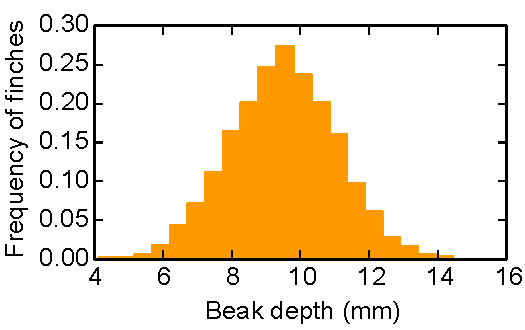
\includegraphics[width=0.43\textwidth]{../images/my-beak-depth-histogram.pdf}

    \vspace{-0.2cm}
    \begin{description}
        \item[Environment:]
            Severe drought---only plant species with large, hard seeds grow;
            large-beaked birds are better at eating these.
    \end{description}

    \vspace{-0.2cm}
    \begin{enumerate}
            \small
        \item Draw the distribution of beak depth in the population after the
                drought.
        \item What happens to the mean and variation of beak depth in the
                population? Why?
            \nbox{\tiny The mean increases while variation decreases; because
                individuals with one ``extreme'' phenotype (large beaks) have
                more offspring}
        \item What happens to genetic variation of beak-depth genes?
            \nbox{\tiny Decreases}
        \item What do we call this mode of selection? Why?
            \nbox{\tiny Directional selection; average phenotype changes in one
                direction}
    \end{enumerate}
\end{adjustwidth}
\end{frame}

\clickerslide{
\begin{frame}
    \begin{clickerquestion}
        \item What happens to the frequencies of alleles associated with beak
            depth during the drought?
        \begin{clickeroptions}
            \item Allele frequencies do not change.
            \item Frequency of alleles associated with large beak size
                increase; frequency of alleles associated with small beak
                size increase.
            \item Frequency of alleles associated with large beak size
                decrease; frequency of alleles associated with small beak
                size decrease.
            \item \clickeranswer{Frequency of alleles associated with large
                    beak size increase; frequency of alleles associated with
                    small beak size decrease.}
            \item Evolution happens.
        \end{clickeroptions}
    \end{clickerquestion}
\end{frame}
}

\begin{frame}[t]
\begin{adjustwidth}{-1.5em}{-1.5em}
    \small
    \vspace{-0.3cm}
    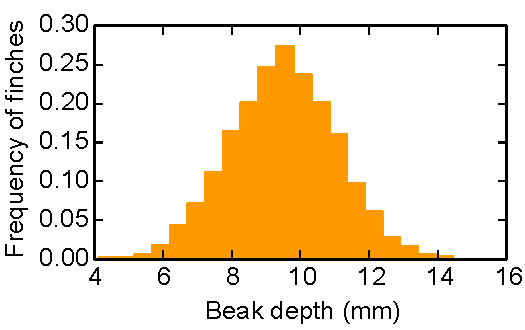
\includegraphics[width=0.43\textwidth]{../images/my-beak-depth-histogram.pdf}

    \vspace{-0.2cm}
    \begin{description}
        \item[Environment:]
            Environment changes such that only plant species with medium-sized
            seeds grow; birds with medium-sized beaks are better at
            eating these.
    \end{description}

    \vspace{-0.2cm}
    \begin{enumerate}
        \item Draw the distribution of beak depth in the population after
            selection in this new environment.
        \item What happens to the mean and variation of beak depth in the
                population? Why?
            \nbox{\tiny The mean stays about the same while variation decreases;
                because individuals with average beak size have more offspring}
        \item What happens to genetic variation of beak-depth genes?
            \nbox{\tiny Decreases}
        \item What do we call this mode of selection? Why?
            \nbox{\tiny Stabilizing selection; individuals that deviate from the
                mean are selected against}
    \end{enumerate}
\end{adjustwidth}
\end{frame}

\clickerslide{
\begin{frame}
    \begin{clickerquestion}
        \item What happens to the frequencies of alleles associated with beak
            depth when only medium-sized seeds are available?
        \begin{clickeroptions}
            \item Allele frequencies do not change.
            \item Frequency of alleles associated with: large beak size
                increase, small beak size decrease, medium beak size increase.
            \item \clickeranswer{Frequency of alleles associated with: large
                    beak size decrease, small beak size decrease, medium beak
                    size increase.}
            \item Frequency of alleles associated with: large beak size
                increase, small beak size increase, medium beak size decrease.
        \end{clickeroptions}
    \end{clickerquestion}
\end{frame}
}

\begin{frame}[t]
\begin{adjustwidth}{-1.5em}{-1.5em}
    \small
    \vspace{-0.3cm}
    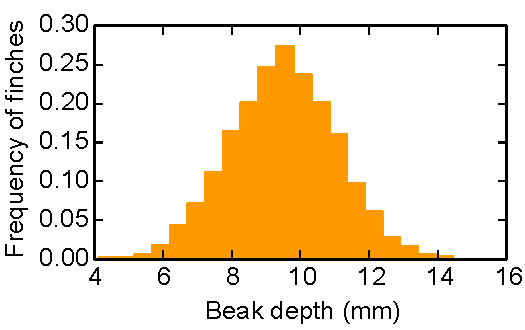
\includegraphics[width=0.43\textwidth]{../images/my-beak-depth-histogram.pdf}

    \vspace{-0.2cm}
    \begin{description}
        \item[Environment:]
            Environment changes such that only plant species with small and
            large seeds grow; birds with medium-sized beaks are
            inefficient at eating either.
    \end{description}

    \vspace{-0.2cm}
    \begin{enumerate}
        \item Draw the distribution of beak depth in the population after
            selection in this new environment.
        \item What happens to the mean and variation of beak depth in the
                population? Why?
            \nbox{\tiny The mean stays about the same while variation increases;
                because individuals with both ``extreme'' beak sizes have more
                offspring}
        \item What happens to genetic variation of beak-depth genes?
            \nbox{\tiny Tends to increase}
        \item What do we call this mode of selection? Why?
            \nbox{\tiny Disruptive selection; individuals with mean phenotype are
                selected against}
    \end{enumerate}
\end{adjustwidth}
\end{frame}

\clickerslide{
\begin{frame}
    \begin{clickerquestion}
        \item What happens to the frequencies of alleles associated with beak
            depth when only ``extreme''-sized seeds are available?
        \begin{clickeroptions}
            \item Allele frequencies do not change.
            \item Frequency of alleles associated with: large beak size
                increase, small beak size decrease, medium beak size increase.
            \item Frequency of alleles associated with: large beak size
                decrease, small beak size decrease, medium beak size increase.
            \item \clickeranswer{Frequency of alleles associated with: large
                    beak size increase, small beak size increase, medium beak
                    size decrease.}
            \item There is selection against indivduals with mean phenotype.
        \end{clickeroptions}
    \end{clickerquestion}
\end{frame}
}

\clickerslide{
\begin{frame}
    \begin{clickerquestion}
        \item If the environment on the island changed and NONE of the alleles
            present conferred high fitness, what would happen?
        \begin{clickeroptions}
            \item \clickeranswer{Average fitness in the population would
                    decrease.}
            \item The population will go extinct.
            \item Allele frequencies do not change.
            \item Average beak depth in the population decreases.
            \item Selection will favor ``strong'' birds.
        \end{clickeroptions}
    \end{clickerquestion}
\end{frame}
}

\clickerslide{
\begin{frame}
    \begin{clickerquestion}
        \item What will happend to the size of beaks in the population of
            ground finches in the future?
        \begin{clickeroptions}
            \item They will continue to get smaller (and pointier).
            \item They will continue to get smaller, but should eventually
                begin to get wider as well.
            \item \clickeranswer{It depends on changes in the environment.}
            \item They may fluctuate in size and shape, but will remain roughly
                constant over the long term (no net change).
        \end{clickeroptions}
    \end{clickerquestion}
\end{frame}
}

\begin{comment}
\begin{frame}
    \frametitle{Directional selection}
    \begin{columns}
        \column{0.5\textwidth}
        \begin{center} 
            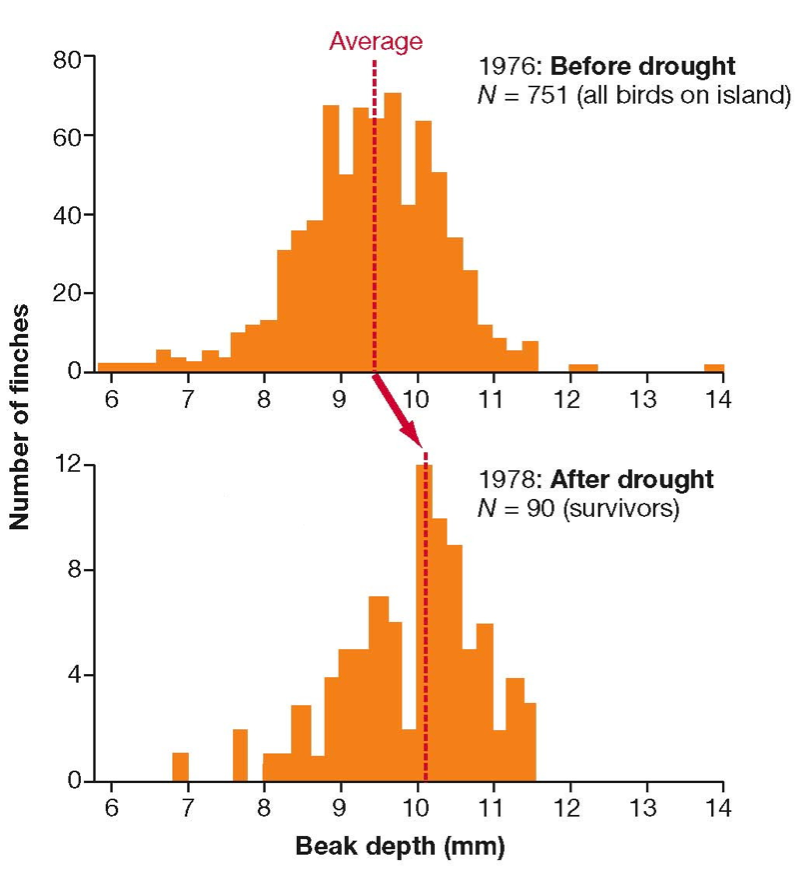
\includegraphics[height=1.1\textheight]{../images/finch-beak-size-histogram.png}
        \end{center}

        \column{0.5\textwidth}

        \uncover<2->{
        \begin{enumerate}
            \item What is ``directional'' about directional selection?
                \nbox{\tiny Mean phenotype changes in one direction}

            \item What happens to overall genetic variation?
                \nbox{\tiny Decreases}

            \item Do allele frequencies change? Explain.
                \nbox{\tiny Yes---alleles associated with small beak size decrease
                    in frequency; alleles associated with large beak size
                    increase in frequency}

            \item If drought conditions continued, would overall variation
                eventually NOT be normally distributed?
                \nbox{\tiny No---variation would be reduced, but independent
                    assortment, recombination, and mutation would continue to
                    generate variation}

            \item If the environment changed and NONE of the alleles present
                conferred high fitness, what would happen?
                \nbox{\tiny Average fitness in the population would decrease;
                    population might go extinct}
        \end{enumerate}
        }
    \end{columns}

\end{frame}
\end{comment}

% \begin{frame}
%     \frametitle{Some information about Exam 1}
%     \begin{itemize}
%         \item We will send you an annotated key with details about
%             grading---read it CAREFULLY
%         \item The regrade policy is posted in the Course Policies
%             materials---read it CAREFULLY
%         \item LEARN from exams---understand why you lost points, what did and
%             did not work about your preparation, and which concepts you are
%             still weak on \ldots so you don't repeat errors
%     \end{itemize}
% \end{frame}

\end{document}

